%!TEX root = main.tex

\section{Evaluation of user influence estimation}
\label{sec:evaluation-influence}

%!TEX root = main.tex

\begin{figure}[tb]
	\centering
%	\newcommand\myheight{0.125}
	\newcommand\myheight{0.171}
	\subfloat[] {
		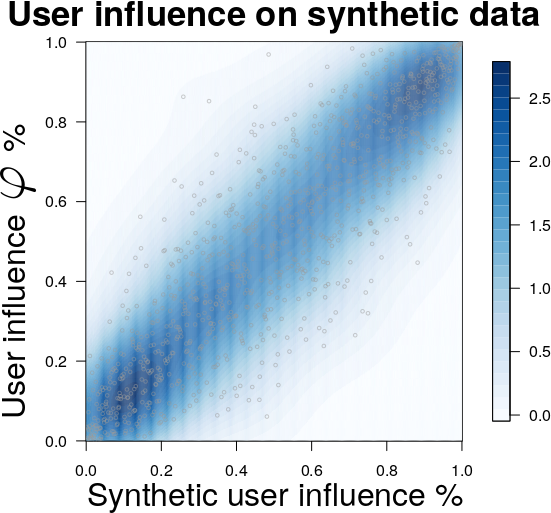
\includegraphics[height=\myheight\textheight]{synthetic-user-influence}
		\label{subfig:artificial-compare}
	}
	\subfloat[] {
		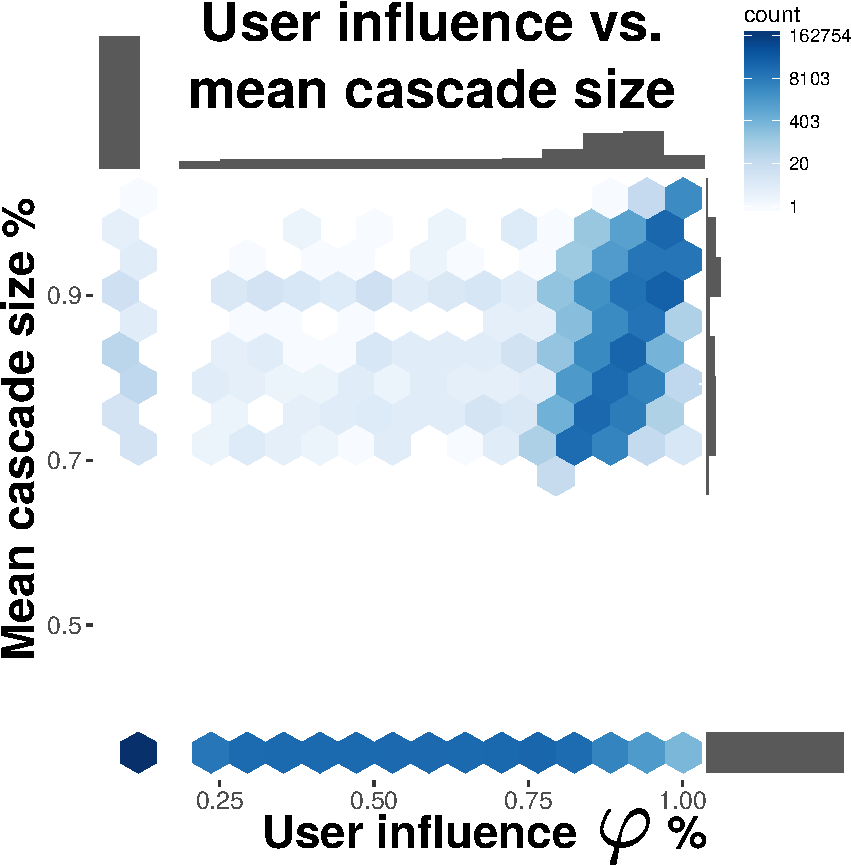
\includegraphics[height=\myheight\textheight]{influence-vs-mcsize}
		\label{subfig:mean-cascade-size}
	}\\
	\subfloat[] {
		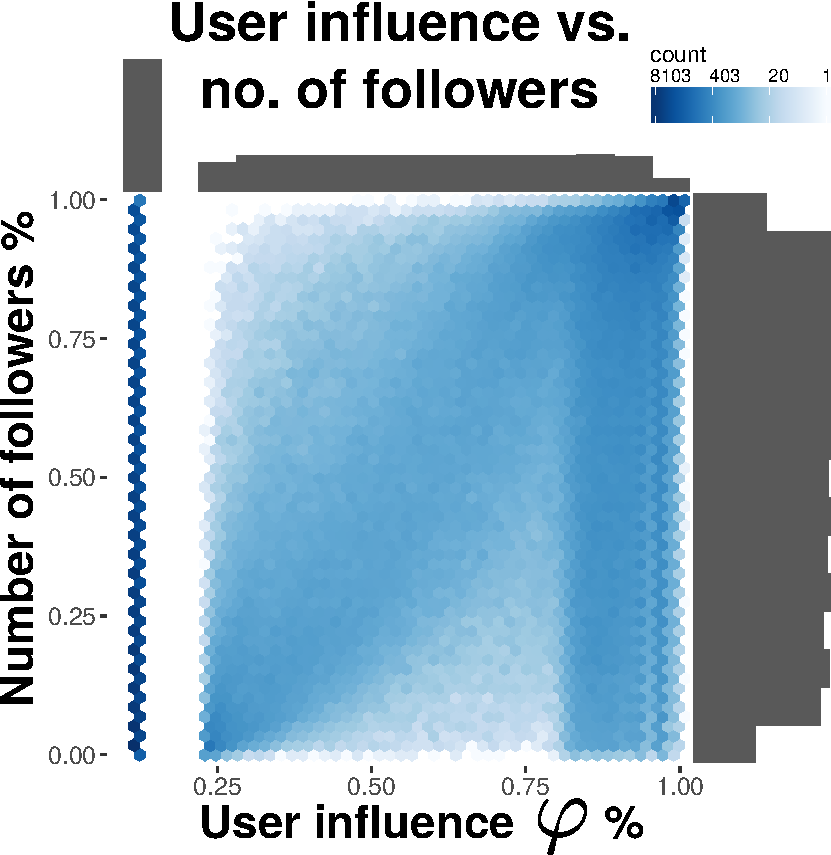
\includegraphics[height=0.19\textheight]{influence-vs-followersCount}
		\label{subfig:no-followers}
	}
%	\subfloat[] {
%		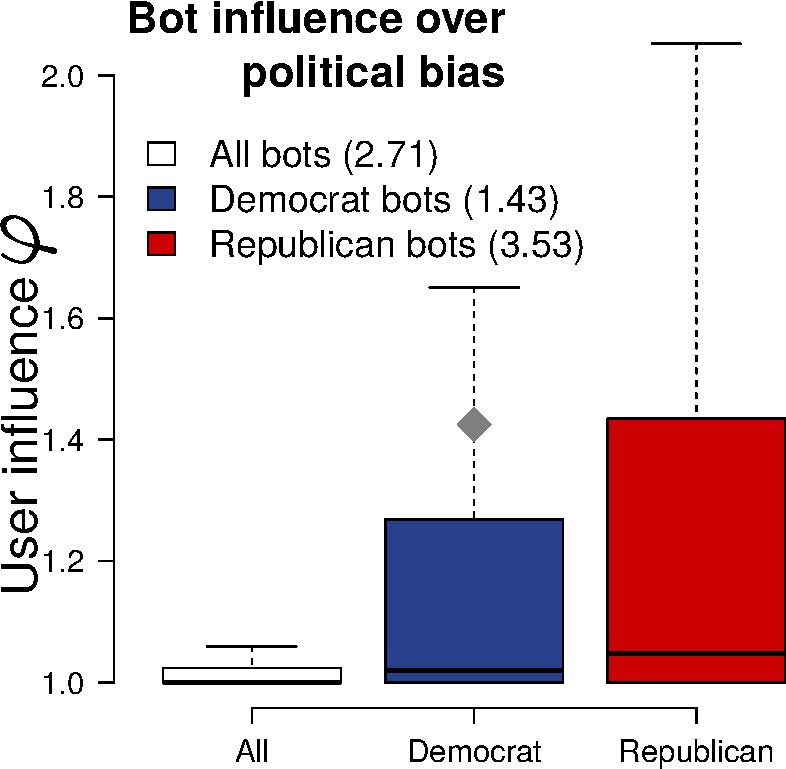
\includegraphics[height=\myheight\textheight]{BOTS_boxplot-influence-vs-political-bias}
%	}
	\caption{ 
		Evaluation of the user influence measure.
		\textbf{(a)} 2D density plot (shades of blue) and scatter-plot (gray circles) of user influence against the ground truth on a synthetic dataset.
		\textbf{(b)(c)} Hexbin plot of user influence percentile (x-axis) against mean cascade size percentile (b) and the number of followers (c) (y-axis) on \debate.
		The color intensity indicates the number of users in each hex bin.
		1D histograms of each axis are shown using gray bars.
		Note $72.3\%$ of all users that initiate cascades are never retweeted.
	}
%	\label{fig:holdout-ll}
%	\captionmoveup
\end{figure}

%!TEX root = main.tex

\begin{figure*}[htbp]
	\centering
	\newcommand\myheight{0.131}
	\subfloat[] {
		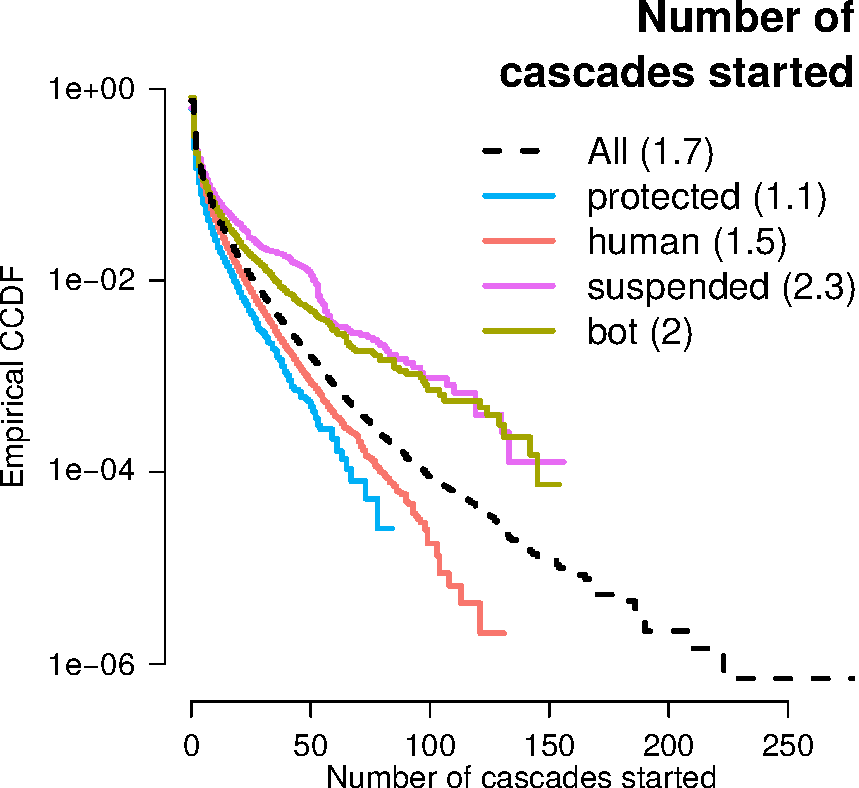
\includegraphics[height=\myheight\textheight]{bot-a-number-of-diffusions}
		\label{subfig:no-cascades}
	}
	\subfloat[] {
		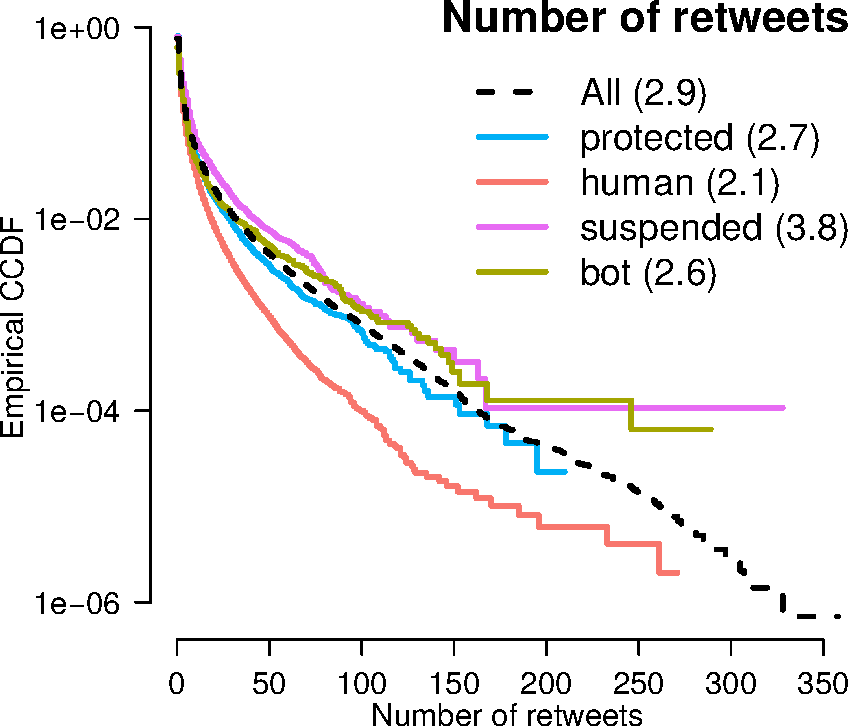
\includegraphics[height=\myheight\textheight]{bot-b-number-of-retweets}
		\label{subfig:no-retweets}
	}
	\subfloat[] {
		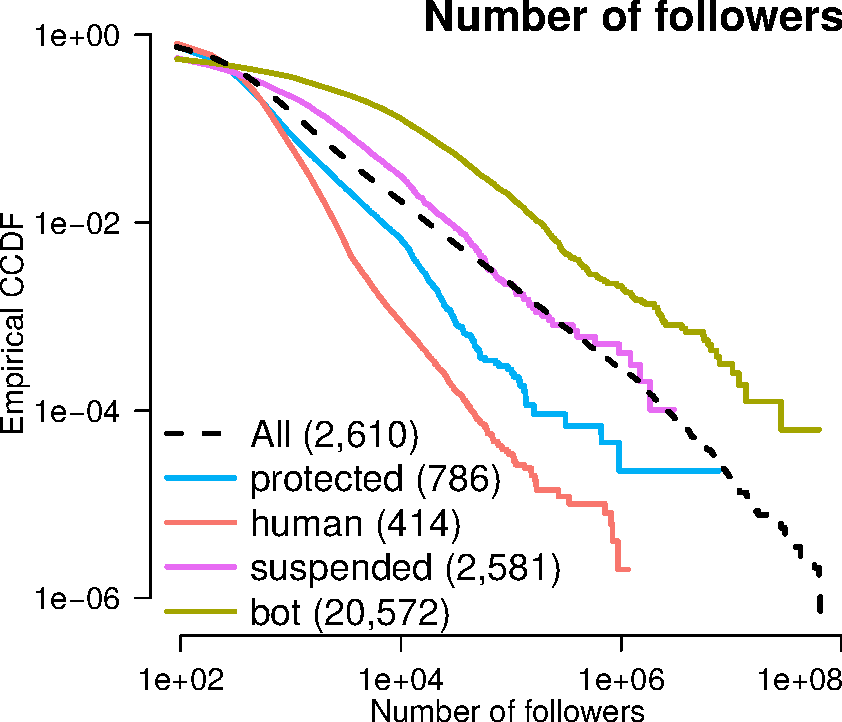
\includegraphics[height=\myheight\textheight]{bot-c-followers-count-CCDF}
		\label{subfig:numfolowers-CCDF}
	}
	\subfloat[] {
		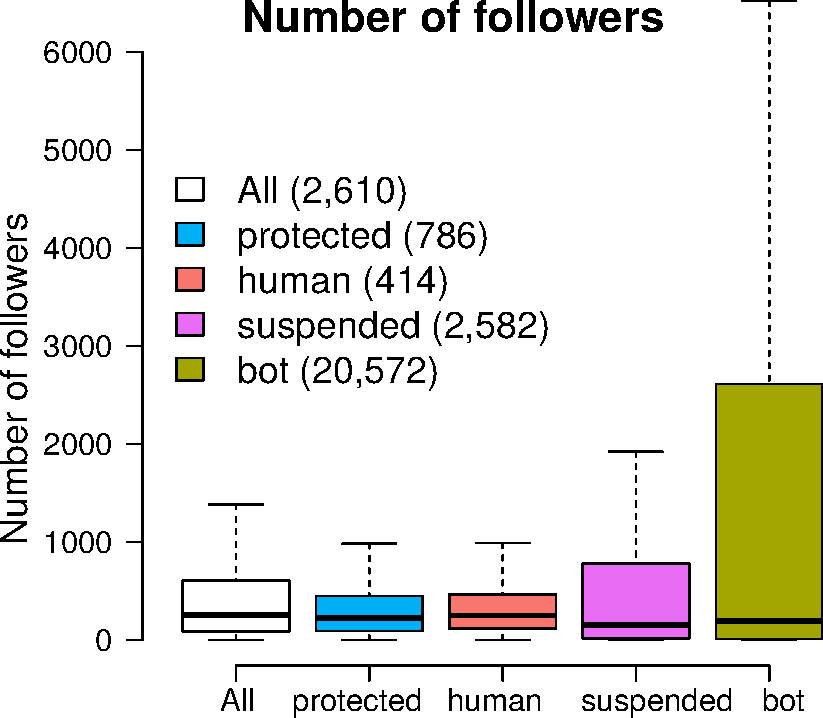
\includegraphics[height=\myheight\textheight]{bot-d-followers-count-boxplot}
		\label{subfig:numfolowers-boxplot}
	}
	\subfloat[] {
		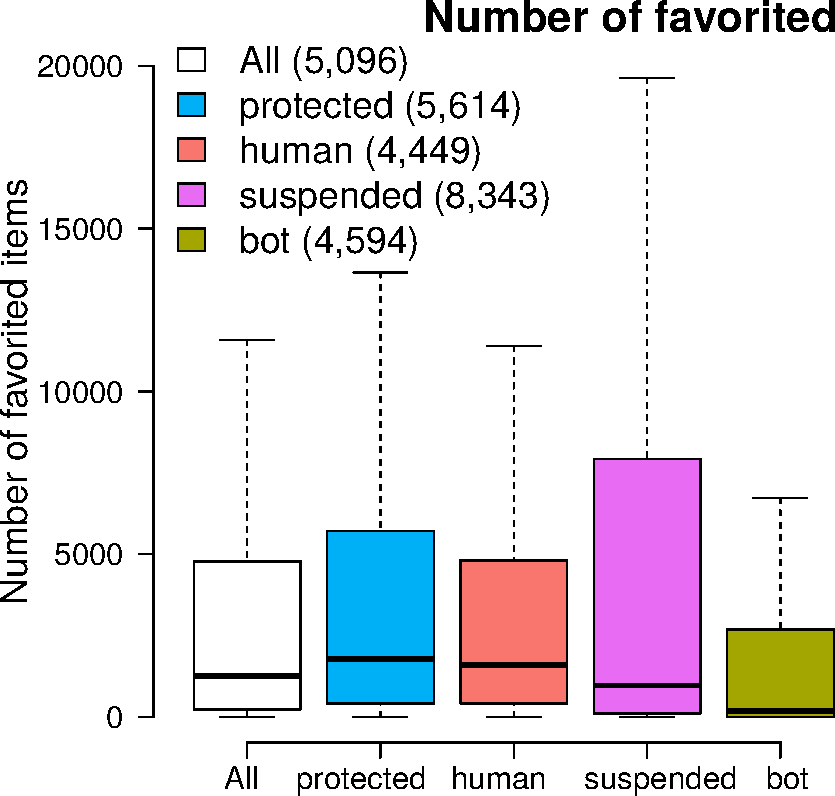
\includegraphics[height=\myheight\textheight]{bot-e-favorites-count}
		\label{subfig:numfavorited}
	}
	\caption{ 
		Profiling behavior of the \Protected, \Human, \Suspended and \Bot populations in the \debate dataset.
		The numbers in parentheses in the legend are mean values.
		\textbf{(a)} CCDF of the number of Twitter diffusion cascades started.
		\textbf{(b)} CCDF of the number of retweets. 
		\textbf{(c)(d)} CCDF (c) and boxplots (d) of the number of followers. 
		\textbf{(e)} Number of items favorited.
	}
	\label{fig:bot-profiling}
%	\captionmoveup
\end{figure*}

%\verify{RJA comment: I was initially wondering if it is necessary to have "$\varphi(u)$ \%" in the figures, thinking it could just be stated in 4.3 that it is normalised (percentiles) and then can just use $\varphi(u)$ throughout. But then I realised that e.g. in Figure 7 the means of unnormalised influence are presented. So I've slightly modified text in 4.3 to highlight we use both.}

In this section, we evaluate our proposed algorithm and measure of user influence.
In Sec~\ref{subsec:ground-truth}, we evaluate on synthetic data against a known ground truth.
In Sec.~\ref{subsec:two-alternatives}, we compare the $\varphi(u)$ measure (defined in Sec.~\ref{subsec:user-influence-measure}) against two alternatives: the number of followers and the mean size of initiated cascades.

\subsection{Evaluation of user influence}
\label{subsec:ground-truth}

%\textbf{Influence is unobserved in real data.}
Evaluating user influence on real data presents two major hurdles.
The first is the lack of ground truth, as user influence is not directly observed.
%While it is possible to manually assess influence, this approach does not scale to the 1.5M users in our dataset.
The second hurdle is that the diffusion graph is unknown, which renders impossible comparing to state-of-the-art methods which require this information (e.g. ConTinEst~\cite{Du2013}).
%Current state of the art methods for uncovering the diffusion structure (e.g. NetInf~\cite{gomez2010inferring}) do not scale to the number of users in our dataset.
%This is because these methods assume a large number of cascades occurring in a rather small social neighborhood.
%
%\verify{RJA comment: The above paragraph is very interesting and I wonder if some of it could be moved into Section 2.1 since there are general points about what is influence, how to measure it etc, and it covers some of the points made in 2.1, but in a different way.  But regardless of position of the material, I have some clarifying questions.  I'm trying to pose the questions that someone who knows about social influence but not these techniques directly may ask. To make this as efficient as possible I'm going to attempt to re-write the above paragraph so you see how I understand it and where misunderstanding may be arising.
%
%Evaluating user influence on real data presents three major hurdles.
%The first is the lack of ground truth, as user influence is not directly observed: in general it is not feasible nor even meaningful to ask people "who are you influenced by?" or "who do you influence?" and this infeasibility is compounded in the context of thousands of users participating in debate related activity on Twitter.
%Given that user influence is not directly observable, interest (especially in the context of social media) has turned to estimating or inferring influence based on a user's contribution to the diffusion of information.
%However in general there will be many diffusion trees that need to be taken account of and so the second hurdle is the need to infer the underlying or latent social network that generated the diffusion trees, and influence is then computed over that social network. This is the approach used by state-of-the-art methods such as ConTinEst~\cite{Du2013}. In the case of user influence on Twitter, we are presented with a third hurdle: we do not have the complete retweet cascade data.
%Current state of the art methods for uncovering the diffusion structure (NetInf and its extension~\cite{gomez2010inferring,gomez2013structure}) do not scale to the number of users in our dataset.
%This is because these methods assume a large number of cascades occurring in a rather small social neighborhood.
%}
%
%\verify{RJA comment: There are in fact two types of latent structure that we are dealing with our particular example. First we do not have the complete diffusion tree data and so we need to deal with this by evaluating all of the possible diffusion scenarios. Second, even if we had complete diffusion tree data we still do not know the latent \emph{social network} which has generated the diffusion trees.}
%In this section, we reproduce ConTinEst's evaluation against a known ground truth on a synthetic dataset.
In this section, evaluate our algorithm against a known ground truth on a synthetic dataset, using the same evaluation approach used for ConTinEst.

\textbf{Evaluation on synthetic data.}
%We compare against ConTinEst~\cite{Du2013} on a synthetic dataset.
We evaluate on synthetic data using the 
%We follow the synthetic data evaluation 
protocol previously employed in~\cite{Du2013}.
We use the simulator in \cite{Du2013} to generate an artificial social network with 1000 users.
We then simulate 1000 cascades through this social network, starting from the same initial user.
The generation of the synthetic social network and of the cascades is detailed in the online supplement~\cite[annex~C]{supplemental}.
%\ref{si-sec:generation-artificial}
Similar to the retweet cascades in \debate, each event in the synthetic cascades has a timestamp and an associated user.
Unlike the real retweet cascades, we know the real diffusion structure behind each synthetic cascade.
%We compute the synthetic user influence as performed in ConTinEst~\cite{Du2013}.
For each user $u$, we count the number of nodes reachable from $u$ in the diffusion tree of each cascade.
We compute the influence of $u$ as the mean influence over all cascades.
ConTinEst~\cite{Du2013} has been shown to asymptotically approximate this synthetic user influence.

%\textbf{Results.}
We use our algorithm introduced in Sec.~\ref{subsec:user-influence-mt} on the synthetic data, to compute the measure $\varphi(u)$ defined in Eq.~\ref{eq:user-infl-casin}.
%We set the parameter of the temporal decay at $r = 6.8 \times 10^{-4}$, determined using linear search on a sample of 20 real retweet diffusions (details in the online supplement~\cite[annex~D]{supplemental}).
We plot in Fig.~\ref{subfig:artificial-compare} the 2D scatter-plot and the density plot of the synthetic users, with our influence measure $\varphi$ on the y-axis and the ground truth on the x-axis (both in percentiles).
Visibly, there is a high agreement between the two measures, particularly for the most influential and the least influential users.
The Spearman correlation coefficient of the raw values is $0.88$.
This shows that our method can output reliable user influence estimates in the absence of any information about the structure of the diffusions.

\subsection{Comparison with other influence metrics}
\label{subsec:two-alternatives}

We compare the influence measure $\varphi(u)$ against two alternatives that can be computed on \debate.

%\textbf{Mean size of initiated cascades} (of a user $u$) is the average number of users reached by content emitted by $u$ and it represents by definition the user influence~\cite{Du2013}.
%\verify{RJA comment: I don't agree with the above statement (note: haven't read Du et al....). I think it represents *one* definition of user influence but not *the* definition of user influence (if it did, then we'd be using it rather than the complicated approach we use here). I think "content emitted by u" is confusing because in fact we are talking about original tweets here, not retweets. How about we say something like: 

\textbf{Mean size of initiated cascades} (of a user $u$) is the average number of users reached by original content authored by $u$.
% and it is one definition user influence~\cite{Du2013}. 
It should be noted that this measure does not capture $u$'s role in diffusing content authored by someone else.
%}
In the context of Twitter, mean size of initiated cascades is the average number of users who retweeted an original tweet authored by $u$: we compute this for every user in the \debate dataset, and we plot it against $\varphi(u)$ in Fig.~\ref{subfig:mean-cascade-size}.
Few users have a meaningful value for mean cascade size: 
$55\%$ of users never start a cascades (and they are not accounted for in Fig.~\ref{subfig:mean-cascade-size}); 
out of the ones that start cascades $72.3\%$ are never retweeted and they are all positioned at the lowest percentile (shown by the 1D histograms in the plot).
%(they all have an equal mean cascade rank of $36.1\%$ on the y-axis of the figure).
%\TODO{RJA}{I think "meaningful value" needs to be clarified. If I authored a single original tweet but no-one retweeted me, then the mean cascade size would be 0 and that is meaningful, I think? However if I never authored an original tweet then I can see that mean cascade size is not computable for me.  Relatedly, the text above implies that $45\%$ of users start a cascade (i.e. author an original tweet) but that doesn't correspond to "very few" and also it doesn't really match up with the histogram on vertical axis.  Or now I'm thinking that you've lumped the users who never started a cascade with those who did start a cascade but it has size 0 because no-one retweeted. I don't understand what is meant by mean cascade rank. }
%
It is apparent that the mean cascade size metric detects the influential users that start cascades, and it correlates with $\varphi(u)$.
However, it misses highly influential users who never initiate cascades, but who participate by retweeting. Examples are user \textit{@SethMacFarlane} (the actor and filmmaker Seth MacFarlane, 10.8 million followers) or user \textit{@michaelianblack} (comedian Michael Ian Black, 2.1 million followers), both with $\varphi$ in the top $0.01\%$ most influential users.

\textbf{Number of followers} is one of the simplest measures of direct influence used in literature~\cite{Mishra2016,Zhao2015}.
While being loosely correlated with $\varphi(u)$ (visible in Fig.~\ref{subfig:no-followers}, Pearson $r = 0.42$), it has the drawback of not accounting for any of the user actions, such as an active participation in discussions or generating large retweet cascades.
For example, user \textit{@PoliticJames} (alt-right and pro-Trump, 2 followers) emitted one tweet in \debate, which was retweeted 18 times and placing him in the top $1\%$ most influential users.
Similarly, user \textit{@tiwtter1tr4\_tv} (now suspended, 0 followers) initiated a cascade of size 58 (top $1\%$ most influential).
Interestingly, half of the accounts scoring on the bottom $1\%$ by number of followers and top $1\%$ by influence are now suspended or have very high botness scores.

%\verify{RJA comment: The evaluation section is really useful for illustrating how our measure of influence can capture what number of followers and number of retweets (received) doesn't. This is just a comment, not for inclusion...}